\documentclass[11pt]{article}
\usepackage[left=3cm, right=3cm, top=2cm, bottom=2cm]{geometry}

\usepackage{verbatim}
\usepackage{afterpage}
\usepackage{graphicx}
\usepackage{amsmath}
\usepackage{amsfonts}
\usepackage{lineno}
\usepackage{setspace}
\usepackage{float}
\usepackage[comma]{natbib}
\graphicspath{{../Results/}}

\newcommand{\reporttitle}{Linear Type I Functional Responses are Unrelated to Feeding Strategy}
\newcommand{\reportauthor}{Luke Swaby}
\newcommand{\reportcid}{01980806}
\newcommand{\words}{2765}
\newcommand{\degreetype}{Master of Science}



\begin{document}
	\bibliographystyle{agsm}
	\setcitestyle{authoryear,open={(},close={)}}

    \onehalfspacing
    % Last modification: 2015-08-17 (Marc Deisenroth)
\begin{titlepage}
    
    \newcommand{\HRule}{\rule{\linewidth}{0.5mm}} % Defines a new command for the horizontal lines, change thickness here
    
    %----------------------------------------------------------------------------------------
    %	LOGO SECTION
    %----------------------------------------------------------------------------------------
    
    
\includegraphics[width = 4cm]{../Writeup/imperial.pdf}\\[0.5cm] 
    
    \center % Center remainder of the page
    
    %----------------------------------------------------------------------------------------
    %	HEADING SECTIONS
    %----------------------------------------------------------------------------------------
    
    \textsc{\Large Imperial College London}\\[0.5cm] 
    \textsc{\large Department of Life Sciences}\\[0.5cm] 
    
    %----------------------------------------------------------------------------------------
    %	TITLE SECTION
    %----------------------------------------------------------------------------------------
    
    \HRule \\[0.4cm]
    { \huge \bfseries \reporttitle}\\ % Title of your document
    \HRule \\[1.5cm]
     
    %----------------------------------------------------------------------------------------
    %	AUTHOR SECTION
    %----------------------------------------------------------------------------------------
    
    \begin{minipage}{0.4\textwidth}
    \begin{flushleft} \large
    \emph{Author:}\\
    \reportauthor \\ [0.5cm] % Your name
    \emph{CID:}\\
    \reportcid % Your name
    \end{flushleft}
    \end{minipage}
    ~
    \begin{minipage}{0.4\textwidth}
    \begin{flushright} \large
    \emph{Words:} \\
    \words \\ [0.5cm] % Word Count
    \emph{Date:} \\
    \today \\ [0.5cm] % Date
    \end{flushright}
    \end{minipage}\\[4cm]
    
    
    %----------------------------------------------------------------------------------------
    %	FOOTER & DATE SECTION
    %----------------------------------------------------------------------------------------
    \vfill % Fill the rest of the page with whitespace
    Submitted in partial fulfillment of the requirements for the MSc degree in
    \degreetype~of Imperial College London\\[0.5cm]
    
    \makeatletter
    \today
    \makeatother


\end{titlepage} % front page
    
    \linenumbers
    
    \renewcommand{\abstractname}{Abstract}
    \begin{abstract}
	A functional response describes the response of a single predator's consumption rate to changes in the population density of its prey. It is thought generally that a relationship exists between functional response type and feeding strategy, a prominent example of which is the conventional association of filter feeders with the type I functional response. Here I test the validity of this association by evaluating the performances of C. S. Holling's type I, II, and III models (as well as a control phenomenological cubic polynomial) across a data set of 308 functional responses spanning a range of feeding types. Multivariate analysis of the model fitting results shows that the proportions of linear type I functional responses found among filter feeders and non-filter feeders in the data set differ insignificantly, and that a type III functional response is in fact the most prevalent among the filter feeders. While ostensibly at odds with the widespread assumption that type I functional responses are exclusive to filter feeders, these results can be partially explained in terms of anomalies in the data set and limitations of the type I model used, leaving grounds to doubt their generalisability without further investigation.    
    \end{abstract}
    
    %%%%%%%%%%%%%%%% INTRODUCTION %%%%%%%%%%%%%%%%
    
    \section{Introduction}
    The term ‘functional response’ refers to a ecological model describing the consumption rate of a single biological consumer as a function of the population density of its target resource \citep{solomon1949natural}. Functional responses encode important behavioural and physiological information about individual organisms and the food webs to which they belong, and have accordingly played an important roll in a wide range of biological fields, ranging from population biology to ethology. As a result, numerous functional response models have been defined in the literature (see \citet{jeschke2002predator} for a review), but since C. S. Holling's seminal 1959 studies these models have been traditionally classified into three types — type I, type II, and type III — each carrying different assumptions about the behaviours at play in the interaction \citep{holling1959a, holling1959b}. 
    
    Most common are type II functional responses  \citep{hassell1976components, begon1996ecology,jeschke2004consumer}. It is assumed here that per capita consumption rates are bounded by the time spent by the consumer to pursue, process and ingest the resource — or, as it's commonly known, the 'handling time'. As such, these curves take a hyperbolic shape with an asymptote where the consumption rate reaches its maximum capacity at high resource densities:
    
    $$
        F(R) = \frac{\alpha R}{1+\alpha hR}     
    $$
    
    where $R$ is the consumption rate, $h$ is the handling time, and $\alpha$ is the rate at which the consumer searches for its prey, or the 'search rate'. These delays can be imposed by, for instance, difficulties subduing large prey \citep{holling1959b,jeschke2002predator,okuyama2015egg} or digestive constraints \citep{jeschke2002predator,van2004digestively}. 
    
    A type III functional response carries all the same assumptions as its type II counterpart, except that its graphical representation features a slight inflection of the curve at lower densities before reaching its saturation point (Fig. 3A). This is caused by the exponentiation of the resource density in both the numerator and denominator of the equation, causing the curve to resemble a sigmoid:
    
    $$
        F(R) = \frac{\alpha R^2}{1+\alpha hR^2}
    $$
    
    This exponent is largely phenomenological, though it has been suggested by some that its consumption-accelerating effect has a mechanistic basis in, for example, 'learning behaviour' \citep{real1977kinetics, holling1965functional} or prey switching \citep{murdoch1977stabilizing}.
    
    Perhaps most specialized of the three is the type I functional response. It is assumed in this model that per capita consumption rates are directly proportional to resource density \citep{holling1959a}. In biological terms, this means that the time taken by the consumer to handle its prey is negligible ($h\approx0$), and the consumption rate is simply equivalent to the rate at which the consumer encounters its prey:
    
    $$
        F(R) = \alpha R
    $$
    
    Since factors like prey size and resistance usually preclude instantaneous capture and consumption, functional responses of this kind are thought to be exclusive to trophic interactions satisfying stringent criteria. More specifically, it has been argued by some that the conditions required to elicit such a response are fulfilled only by passive predators such as suspension feeders, trap-builders, and filter feeders \citep{jeschke2004consumer}.
    
    By reviewing 308 functional responses compiled from the literature, I test the hypothesis that type I functional responses are significantly more prevalent among filter feeders than non-filter feeders, and examine the extent to which this evaluation is influenced by the model comparison approach adopted. I additionally evaluate the performance of a phenomenological model against Holling's functional response models and, subsequently, the performances of all four models accross the data set to examine the relationship between feeding type and functional response more generally.
    
    %%%%%%%%%%%%%%%% METHODS %%%%%%%%%%%%%%%%
    
    \section{Methods}
    
    \subsection{Data}
    The data set reviewed here consists of functional response data collected for 308 consumer-resource interactions from field and laboratory experiments around the world, covering over 240 species from both terrestrial and aquatic habitats. Each response is assigned a unique ID number. Of the 50+ metadata fields, only a small subset are of special interest to this paper: habitat, experiment type (laboratory or field), taxonomy, foraging movement, and movement dimensionality.
    
    Irrelevant fields and problematic data values were filtered out before the model fitting. In particular, any rows with zero values in either the explanatory (resource density) or response (consumption rate) fields were dropped, along with any data sets for which multiple irreconcilable measurement units were used within either field. Terminology was also standardised in the relevant metadata fields to enable more efficient comparative analysis down the line. 
    
    \subsection{Model Fitting}
    
    Both the cubic polynomial and Holling's type I model were fitted using ordinary least squares regression (OLS), with any responses lacking sufficient data points dropped (identified by checking for perfect fits; $R^2=1$). For the non-linear type II and III models, approximate values for their parameters — $h$ and $\alpha$ — were first estimated. Following L. A. \citet{real1977kinetics}, $h$ is assumed to be approximate to $1/F_{max}$ (as $\lim_{R\to\infty}F=1/h$) and $\alpha$ to $F_{max}/R_{half}^{q+1}$ for a given functional response, where $F_{max}$ is the maximum consumption rate,  $R_{half}$ is the resource density at half the maximum consumption rate, $q=0$ for type II and $q=1$ for type III. A Latin Hypercube sample of 30 parameter combinations was then taken from the spaces around these initial estimates, which were then individually plugged into the models and fitted to the data by non-linear least squares regression (NLLS) with an upper time limit of 3 seconds for each ID, after which the fitting ceased (if all parameter combinations had not already been tested) and the combination with the lowest AIC score was recorded as the optimal fit.
    
    \subsection{Analysis}
    
    AIC and BIC values recorded in the model fitting step were used to conduct an information-theoretic model comparison in order to determine the most successful model for each response. The general 'rule of thumb' for such a comparison — for both estimators — is that if the difference between the scores of two models for a particular data set is less than two  (i.e.  $\Delta_i<2$, where $\Delta_i$ is the difference between the score of model $i$ and the lowest score among the set of examined models), then neither is to be considered significantly supported over the other by that data \citep{anderson2004model}. This rule (hereafter denoted 'the Rule of Two') was used here to generate confidence sets of the 'best' models for each functional response in the data set, of the form: $\{M_{i}\;|\:\Delta _{i} < 2,\:i\in\mathbb{N}\}$. Selecting a winning model from among these on the basis of raw AIC/BIC scores alone can be problematic, however \citep{wagenmakers2004aic}, so two approaches were evaluated. In the first, ID's for which any models scored within two units of the lowest (for either estimator) were considered mixed responses and overlooked. On the second, the Rule of Two was dispensed with entirely and the model with the lowest raw AIC/BIC score was accepted as the best, irrespective of the margin by which it won.
    
    The data was then split by feeding type. Following \citet{jeschke2004consumer}, filter feeders were defined broadly to include all suspension feeders, trap-builders and sediment filter feeders. On this definition, the taxonomic information for the ID's was manually examined and split into filter feeders and non-filter feeders. This step set the stage for a general analysis of the relationship between feeding type and functional response along several variables: model type (phenomenological versus mechanistic), information criterion (AIC versus BIC), and selection method (Rule of Two applied versus Rule of Two not applied). 
    
    \subsection{Computing Tools}
    
    The data was prepared for model fitting in R 4.0.3 on account of its convenient data wrangling and exploration packages. The computationally intensive task of model fitting itself was then performed in Python 3 using the \texttt{lmfit} and \texttt{numpy} modules. Python was chosen for this step primarily due its versatility over a broader range of tasks than R, as well as its simple debugging and parallel processing capacities. For the parameter sampling method, Latin Hypercube sampling was chosen over random uniform sampling in order to ensure broader coverage of each parameter space and maximize the probability of finding the global optimum. 
    R was then used once more for plotting and analysis due to its field-specific features in this area.

    %%%%%%%%%%%%%%%% RESULTS %%%%%%%%%%%%%%%%
    
    \section{Results}
    \subsection{Mechanistic vs. Phenomenological Models}
    
    Unsurprisingly, the data demonstrate a strong preference for mechanistic models across the board (Fig. 1). According to both estimators, approximately 95\% of functional responses were best fit by mechanistic models, regardless of feeding type or whether or not the Rule of Two was applied ($p<$0.1e-15 for one-proportion Z-tests in all cases). The Rule of Two proved inconsequential at this stage of the analysis as the number of 'close games' between phenomenological and mechanistic models (i.e. $\Delta_i<2$) was negligible, leading to more-or-less identical model type scoring.
    
    \afterpage{
    \begin{figure}[t!]
	    \centering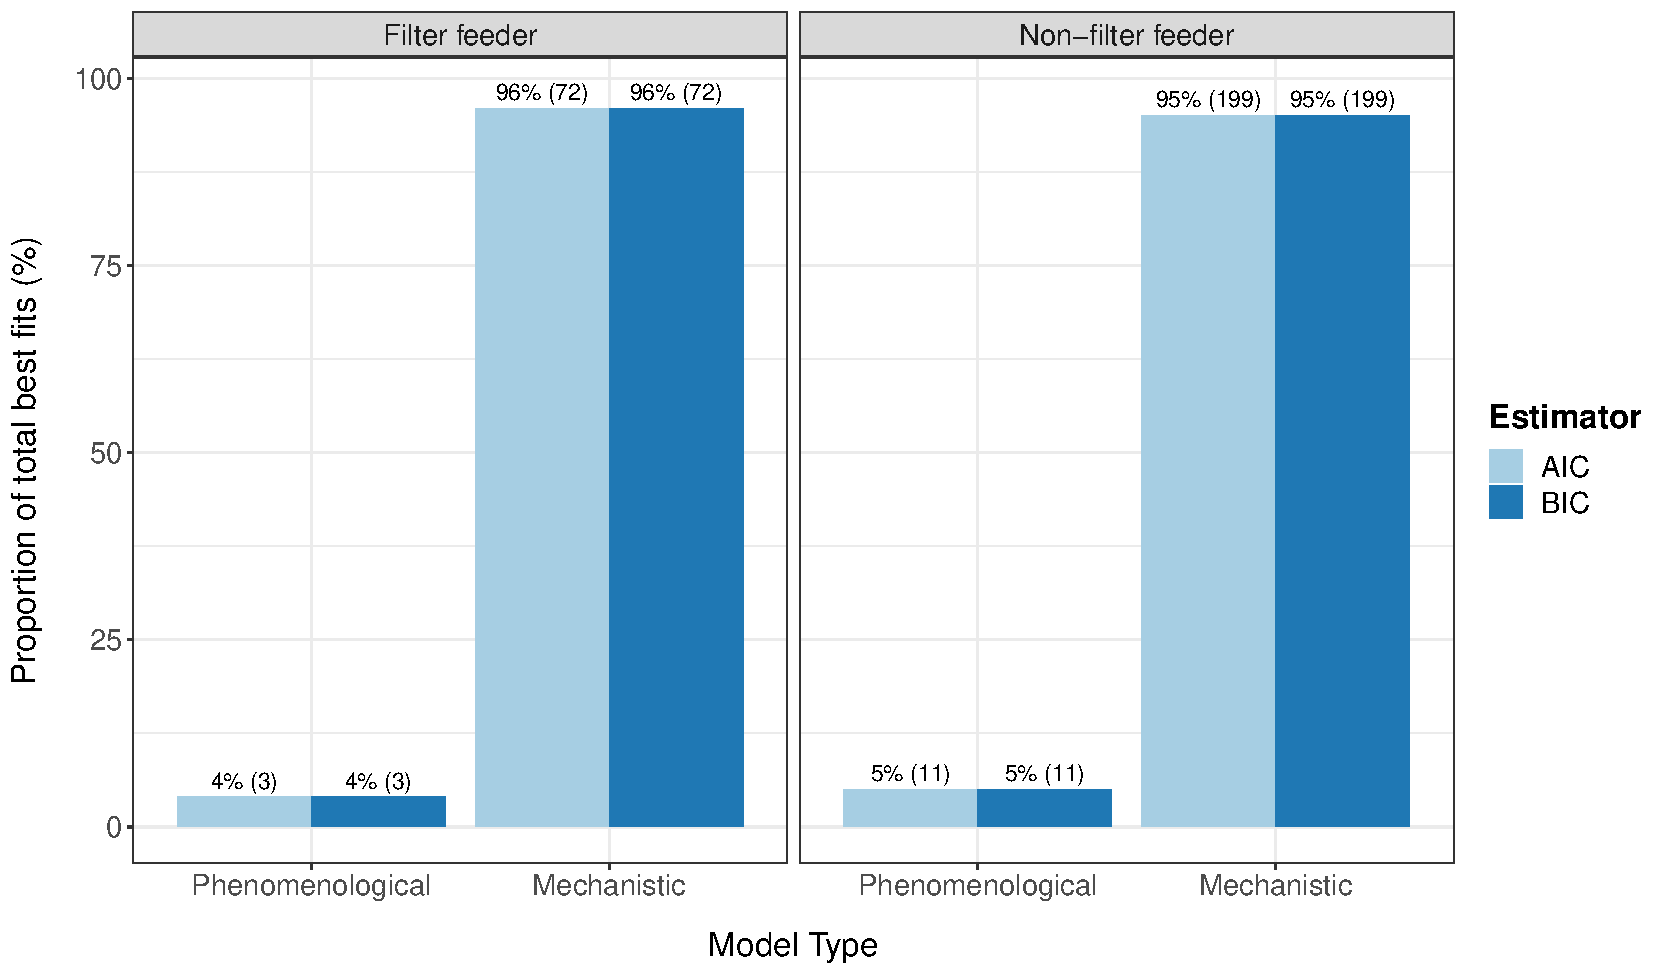
\includegraphics[width=1\textwidth]{TypeComparisonBar.pdf}
	    \caption{Percentage of functional responses best fit by model type.}
    \end{figure}
    }
    
    \subsection{Functional Responses in Filter Feeders}
    
    On the contrary, in the individual model comparison I found substantial differences between model performances depending on the implementation of the Rule of Two (Fig. 2).
    
    \subsubsection{Type I}
    
    Apparently at odds with the observations of \citet{jeschke2004consumer}, I found that if the Rule of Two was ignored then the difference in type I performance between filter feeders and non-filter feeders was statistically insignificant on both the AIC and BIC ($p>0.05$). Interestingly however, whilst the performance gap remained statistically insignificant according to the AIC ($\chi^2=1.7608;\:df=1;\:p>0.1$) it became highly significant according to BIC when the more conservative Rule of Two was employed ($\chi^2=16.617;\:df=1;\:p<0.0001$).
    
    \subsubsection{Types II and III}
    
    Consistent with general consensus \citep{hassell1976components, begon1996ecology}, a type II functional response was most prevalent among non-filter feeders, fitting around 50-70\% of all curves for which there was a definitive best model (Fig. 2). This trend held true irrespective of the implementation of the Rule of Two, with only a slight performance improvement with the rule in place (suggesting a number of mixed responses with type II taking a negligible statistical edge, i.e. $\Delta_i<2$). 
    Furthermore, a significantly higher proportion of type III functional responses were also found among filter feeders than non-filter feeders ($\chi^2=4.0775;\:df=1;\:p<0.05$). 
    
        
    \begin{figure}[t!]
	    \centering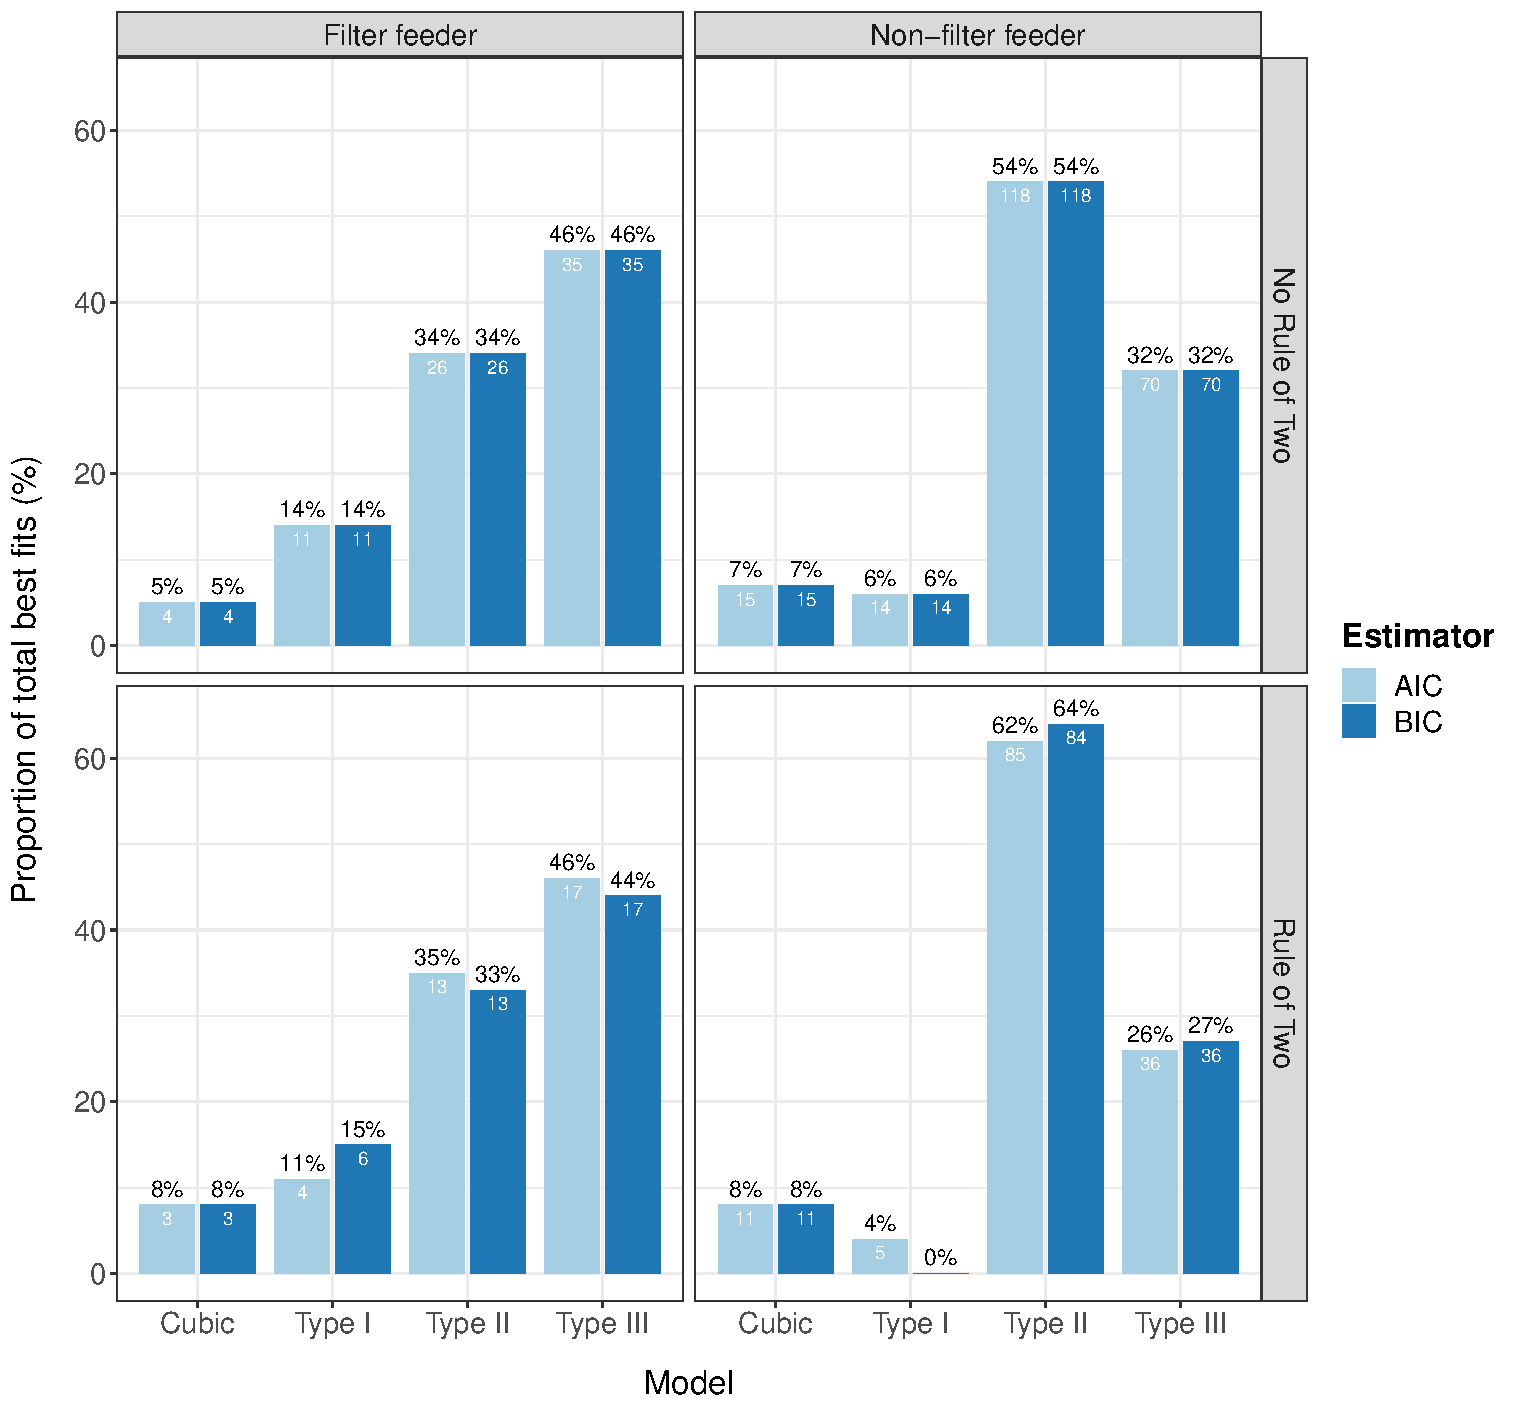
\includegraphics[width=1\textwidth]{ModelComparisonBar.pdf}
	    \caption{Percentage of functional responses best fit by model.}
    \end{figure}
   
    %%%%%%%%%%%%%%%% DISCUSSION %%%%%%%%%%%%%%%%
    
    \section{Discussion}

    From the result that the AIC and BIC significantly disagree on the assignment of type I status to the filter feeders in the data set we may draw some conclusions. Firstly, the majority of functional responses in the non-filter feeder data set that are classified as type I when the Rule of Two is abandoned are likely mixed responses (e.g. type I/II responses), as hypothesized by \citet[p.341]{jeschke2004consumer}. Accordingly, excluding these from the type I classification bracket would probably generate results much closer to those obtained when the Rule of Two was applied, and align our results with Jeschke's conclusion that definitive type 1 functional responses are in fact exclusive to filter feeders.
    
    Given that the BIC typically penalizes model complexity most heavily of the two estimators, it should be noted that the result that the AIC definitively favours the simplest model in cases where the BIC does not is at first glance a counter-intuitive one. However, this is readily explained by the low sample size for these data sets. For each of the non-filter feeder functional responses labelled type I by the AIC under the Rule of Two, the sample size ($N$) is beneath the threshold past which the BIC's per-parameter penalty exceeds that of the AIC (the AIC penalizes by a constant factor of 2, whereas the BIC does so by a factor of $ln(N)$, which is only greater than 2 for sample sizes exceeding 7 as $N \leq 7\implies ln(N)<2$ for $N\in\mathbb{N}$). This parameter tolerance at low sample sizes explains why the BIC scores of Holling's higher order models are being placed within range ($\Delta_i<2$) of the type I model for these curves, and are consequently being overlooked in the Rule of Two analysis as mixed responses. In light of this, it seems sensible to accept the AIC as the more informative estimator here and conclude that there is no significant difference between the proportion of type I functional responses in the filter feeders and non-filter feeders in this data set.
    
    An obvious factor in this result that is worth considering is is the generally low prevalence of type I responses across the data set as a whole. A possible explanation for this is to do with some shortfalls of the model used. Firstly, only linear functional responses were considered type I here. It could be argued, as it was by Jeschke himself (2004), that curves lacking a saturation point as these do simply lack sufficient data to be classified properly and so can't be confidently assigned a functional response type at all. 
    Moreover, it is also generally assumed that the functional response curve must pass through the origin, when it is in fact possible for it to feature a non-zero $y$-intercept if the consumer's diet includes a resource whose densities are not recorded. Of course, to allow a variable y-intercept one would need to include a purely phenomenological constant in the type I model, potentially undermining the biological intelligibility of the results. However, even if one were to ignore this additional feature and furnish the type I model with a saturation point only (for example, $F(R)=min\{\alpha R,\:F_{max}\}$) it is quite possible that a significant number of the curves with sharp inflections at the saturation point that were assigned type II and III status under the models used here (e.g. Fig. 3D) would resolve into type I.
    
    %'The authors suggest that the reason the line does not pass through the origin (coordinates [0,0] on the graph) is that the lemmingsí diet included a constant rate of consumption of mosses, whose biomass measurements were not included in the study.' http://www.tiem.utk.edu/~gross/bioed/bealsmodules/functional1.html
    
    \begin{figure}[t!]
	    \centering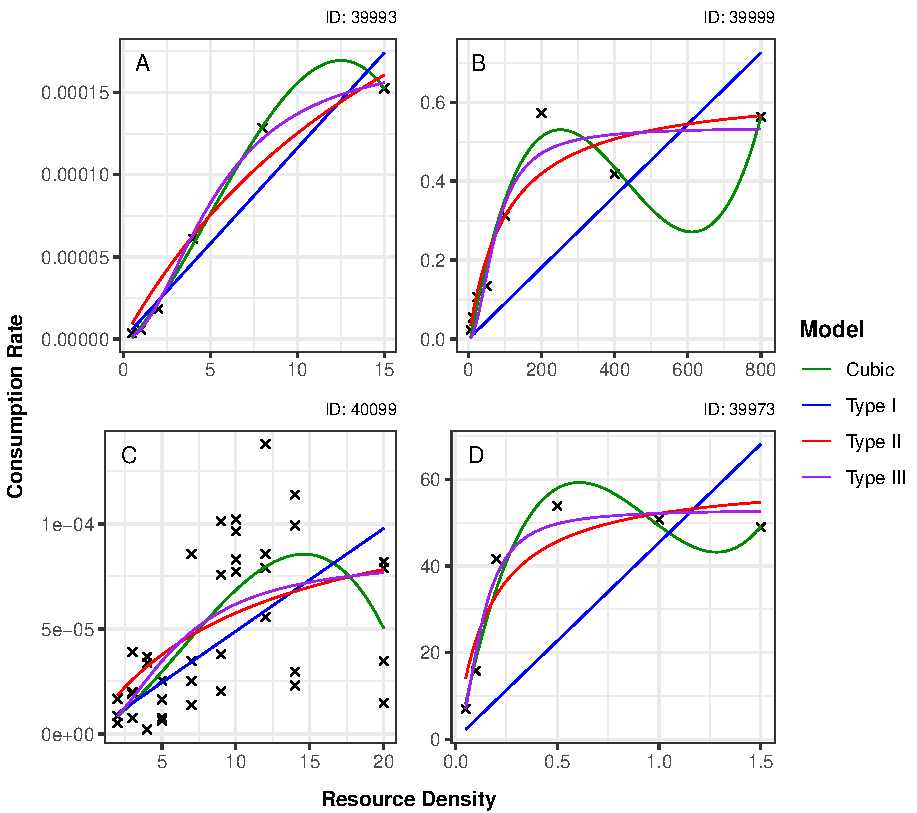
\includegraphics[width=1\textwidth]{TypeIIIFilts.pdf}
	    \caption{Performance of the four models for a sample of IDs.}
    \end{figure}
    
    This consideration covers some ground in explaining the performance gap between the type I model and its higher order counterparts, but leaves unexplained the reversal in performance of the types II and III models between the filter feeder and non-filter feeder data sets. \citet{jeschke2004consumer} speculate that type III responses are typically seen in filter feeders when they lower their filtration rates at low resource densities (p.343). However, there is little evidence to support this in the data. Whilst a substantial number of curves in this set appear to be legitimate type III responses (e.g. Fig. 3A), upon closer inspection it can be seen that many of them are skewed into a sigmoidal shape by single anomalous data points (Fig. 3B) or clusters of unequal replicates (Fig. 3C), making it difficult to draw any reliable conclusions about the true nature of the functional response.
    
    Examination of the corresponding metadata also revealed little of any interest here. The only fields which seemed to exhibit superficial trends — most notably experiment type (100\% of functional responses in this set were recorded in a lab), habitat, consumer foraging movement, and consumer movement dimensionality — differed insignificantly from the overall data set, scoring $p=0.4$, $p=0.06$, $p=0.4$, and $p=0.6$ respectively in $\chi^2$-tests against the data set as a whole. This is perhaps to be expected, as there is no known correlation between any of these broad fields and the specific conditions thought generally to elicit a type III functional response. Perhaps greater field specificity and more information regarding experimental conditions could help clarify whether or not the conditions for type III-relevant behaviours are satisfied to any significant degree in this data set. (For example, it is suggested by \citet{pawar2012dimensionality} that 'habitat structural complexity' could elicit learning behaviour from consumers as they learn to navigate the terrain in search for prey.) However, this is information that we presently do not have.
    
    \section{Conclusions}
    
    All in all, contrary to the observations of \citet{jeschke2004consumer} my results indicate that type I functional responses are not significantly prevalent among the filter-feeders in the data set used, and that the most significant proportion of them are actually of type III. It remains unclear whether this is representative of any generalizable biological trend or just idiosyncrasies in the data and the methods used to collect it. There is little evidence of a biological pattern in the data, but this may be due to the defects of the type I model used. If these were rectified, it is highly possible that a large number of the functional responses labelled type II and III under my analysis would be redefined as type I, and a biological narrative would emerge. Consequently, although we can confidently say that Jeschke's conclusion is not supported by the data with respect to strictly linear type I models, we do not have sufficient grounds to conclusively reject its applicability to type I models in general.

    \newpage
    
    %\bibliographystyle{abbrvnat}
    \bibliography{Biblio}
\end{document}